\documentclass[11pt,letterpaper]{article}

\usepackage[spanish,es-tabla,es-noshorthands]{babel}
\usepackage[margin=2.5cm]{geometry}
\usepackage{graphicx}
\usepackage{booktabs}
\usepackage{tabularx}
\usepackage{float}
\usepackage{caption}
\usepackage{amsmath}
\usepackage{xcolor}
\usepackage{listings}
\usepackage{enumitem}
\usepackage{fancyhdr}
\usepackage[hidelinks]{hyperref}

\graphicspath{{../}}

\definecolor{azuljaveriana}{RGB}{44,86,151}
\definecolor{fondocodigo}{RGB}{246,247,249}
\definecolor{comentario}{RGB}{110,120,130}

\lstset{
  language=Python,
  basicstyle=\ttfamily\scriptsize,
  backgroundcolor=\color{fondocodigo},
  keywordstyle=\color{azuljaveriana}\bfseries,
  commentstyle=\color{comentario}\itshape,
  stringstyle=\color{red!60!black},
  numbers=left, numberstyle=\tiny\color{gray},
  frame=single, rulecolor=\color{gray!40},
  xleftmargin=1.8em, framexleftmargin=1.5em,
  breaklines=true, showstringspaces=false,
  columns=fullflexible, keepspaces=true,
  extendedchars=true, inputencoding=utf8
}

\pagestyle{fancy}
\fancyhf{}
\lhead{\small Sistemas Inteligentes -- Actividad guiada}
\rhead{\small Brayan David Zuluaga}
\cfoot{\thepage}

\setlist{itemsep=2pt}
\captionsetup{font=small,labelfont=bf}

\begin{document}

% ------------------------------------------------------------------ Portada
\begin{titlepage}
  \centering
  \vspace*{2cm}
  {\Large\bfseries Pontificia Universidad Javeriana Cali\par}
  \vspace{0.3cm}
  {\large Facultad de Ingeniería y Ciencias\par}
  \vspace{2.5cm}
  {\color{azuljaveriana}\rule{\linewidth}{1pt}\par}
  \vspace{0.4cm}
  {\huge\bfseries Actividad guiada:\\[0.2cm] Machine Learning supervisado\\ y no supervisado\par}
  \vspace{0.4cm}
  {\color{azuljaveriana}\rule{\linewidth}{1pt}\par}
  \vspace{1cm}
  {\large Clasificación de pacientes con diabetes y segmentación de clientes\\ con datos sintéticos\par}
  \vfill
  {\large\bfseries Brayan David Zuluaga\par}
  \vspace{0.3cm}
  {\large Sistemas Inteligentes\par}
  \vspace{1.5cm}
  {\large Santiago de Cali, octubre de 2026\par}
\end{titlepage}

\tableofcontents
\newpage

% ------------------------------------------------------------------ Intro
\section{Introducción}

En esta actividad trabajé con los dos enfoques clásicos del aprendizaje automático. En la primera parte
armé un conjunto de datos sintético de pacientes y entrené dos clasificadores para predecir si una persona
tiene diabetes. En la segunda parte generé datos de clientes de un supermercado y usé tres algoritmos de
agrupamiento para encontrar segmentos sin decirle al modelo a qué grupo pertenece cada cliente.

Como los datos son sintéticos, tuve control total sobre cómo se generan, lo cual es muy útil: puedo
verificar si los modelos realmente descubren la estructura que yo mismo metí en los datos. Todo se hizo en
Python con NumPy, Pandas, Matplotlib, SciPy y scikit-learn, usando siempre la semilla \texttt{42} para que los
resultados se puedan reproducir.

% ================================================================== PARTE 1
\section{Parte 1: ML supervisado -- predicción de diabetes}

\subsection{Descripción del problema}

La idea es simular la información médica de 2.000 pacientes con cinco variables predictoras: edad, nivel de
glucosa en sangre, índice de masa corporal (IMC), presión arterial y antecedentes familiares. Cada paciente
tiene una etiqueta que dice si tiene diabetes (\emph{Sí}) o no (\emph{No}). Con eso se entrenan dos
algoritmos de clasificación y se compara cuál funciona mejor.

\subsection{Distribuciones seleccionadas}

Escogí cada distribución pensando en que tuviera sentido para la variable que representa:

\begin{table}[H]
\centering
\caption{Distribuciones usadas para las variables predictoras}
\small
\begin{tabularx}{\linewidth}{lllX}
\toprule
\textbf{Variable} & \textbf{Distribución} & \textbf{Parámetros} & \textbf{Por qué} \\
\midrule
Edad (años)            & Normal truncada & $\mu=50,\ \sigma=15$, en $[18, 90]$ & Población adulta, sin edades imposibles \\
Glucosa (mg/dL)        & Normal          & $\mu=100,\ \sigma=20$                & Variable fisiológica simétrica \\
IMC (kg/m$^2$)         & Lognormal       & mediana $=27$, $\sigma_{\log}=0{,}18$ & Siempre positiva y con cola a la derecha \\
Presión arterial (mmHg)& Normal          & $\mu=125,\ \sigma=15$                & Variable fisiológica simétrica \\
Antecedentes familiares& Bernoulli       & $p=0{,}30$                           & Es una variable de sí/no \\
\bottomrule
\end{tabularx}
\end{table}

\paragraph{Regla para construir la etiqueta.} Como los datos son inventados, la etiqueta de diabetes tiene que
salir de una fórmula conocida. Usé un puntaje lineal con ruido que luego paso por una sigmoide:
\begin{equation}
\begin{split}
z = {} & -11{,}5 + 0{,}03\,\text{edad} + 0{,}05\,\text{glucosa} + 0{,}08\,\text{IMC} \\
       & + 0{,}015\,\text{presión} + 1{,}0\,\text{antecedentes} + \varepsilon, \qquad \varepsilon \sim \mathcal{N}(0;\,0{,}75)
\end{split}
\end{equation}
\begin{equation}
p = \frac{1}{1+e^{-z}}, \qquad
\text{diabetes} = \begin{cases} \text{Sí} & \text{si } p \ge 0{,}5 \ (z \ge 0)\\ \text{No} & \text{en otro caso} \end{cases}
\end{equation}
El término de ruido $\varepsilon$ representa factores que no medimos (dieta, actividad física, genética,
etc.). Gracias a ese ruido las clases no quedan perfectamente separadas, que es lo que pasaría con datos reales.

\subsection{Código utilizado para generar los datos}

\lstinputlisting[firstline=63,lastline=138]{../supervisado/supervisado.py}

El código completo (análisis exploratorio, modelos y métricas) está en \texttt{supervisado/supervisado.py}.

\subsection{Análisis exploratorio}

\begin{table}[H]
\centering
\caption{Estadísticas descriptivas ($n = 2.000$)}
\small
\begin{tabular}{lrrrrrrrr}
\toprule
\textbf{Variable} & \textbf{Media} & \textbf{Desv.} & \textbf{Mín.} & \textbf{Q1} & \textbf{Mediana} & \textbf{Q3} & \textbf{Máx.} & \textbf{Asim.} \\
\midrule
Edad          & 50,66  & 14,15 & 18,18 & 40,14  & 50,09  & 60,70  & 89,30  & 0,15 \\
Glucosa       & 100,40 & 19,90 & 38,72 & 86,73  & 100,33 & 113,57 & 161,77 & 0,06 \\
IMC           & 27,50  & 5,02  & 12,25 & 23,93  & 27,10  & 30,35  & 50,28  & 0,58 \\
Presión       & 124,75 & 15,00 & 79,06 & 115,17 & 124,09 & 135,02 & 174,41 & 0,02 \\
Antecedentes  & 0,29   & 0,46  & 0     & 0      & 0      & 1      & 1      & 0,90 \\
\bottomrule
\end{tabular}
\end{table}

Las medias y desviaciones quedaron muy cerca de los parámetros que puse. El IMC es la única continua con
asimetría positiva clara (0,58), lo cual es justo lo que se espera de una lognormal.

\begin{figure}[H]
\centering
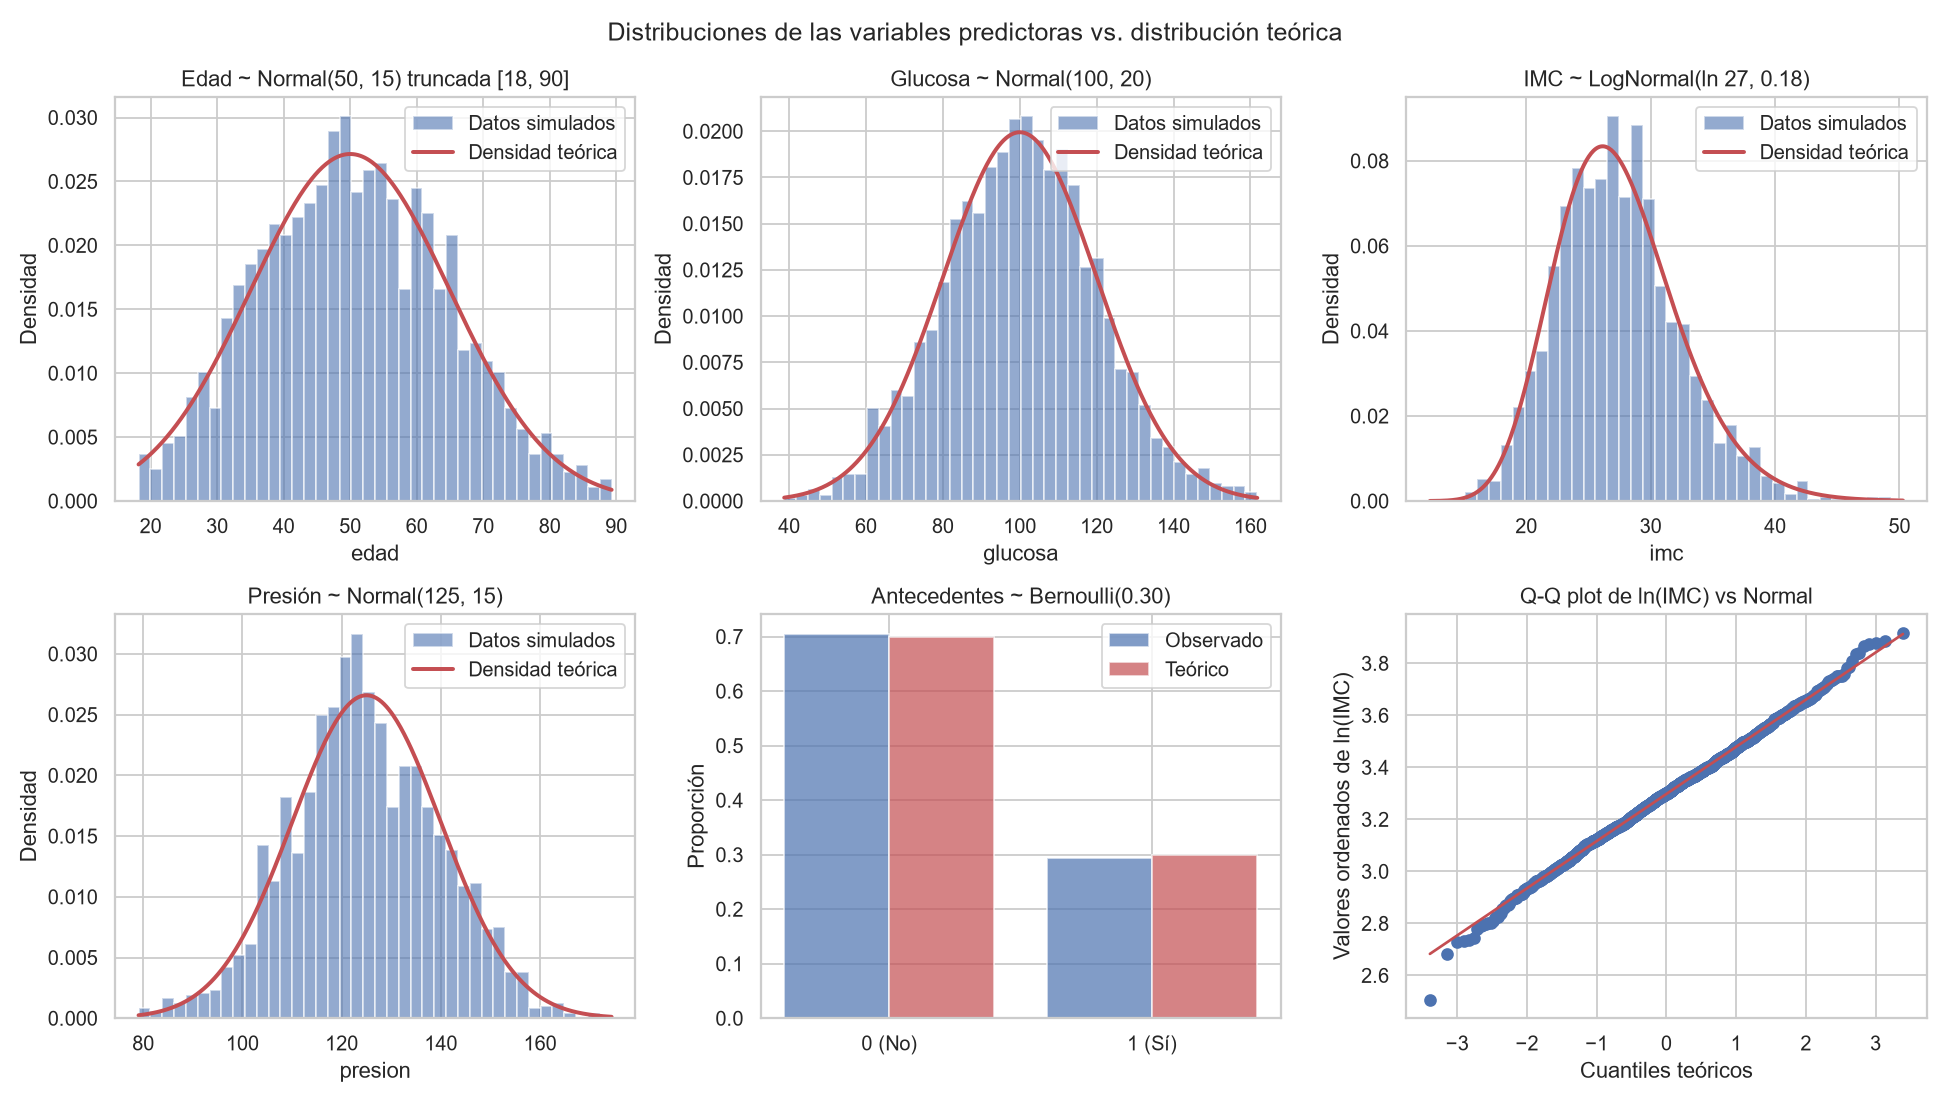
\includegraphics[width=\linewidth]{supervisado/figuras/histogramas_teoricos.png}
\caption{Histogramas de cada variable con la densidad teórica superpuesta}
\end{figure}

\begin{figure}[H]
\centering
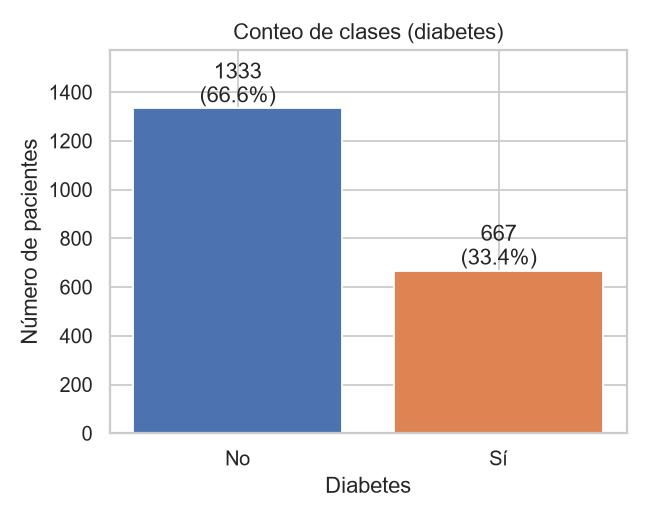
\includegraphics[width=0.48\linewidth]{supervisado/figuras/conteo_clases.png}
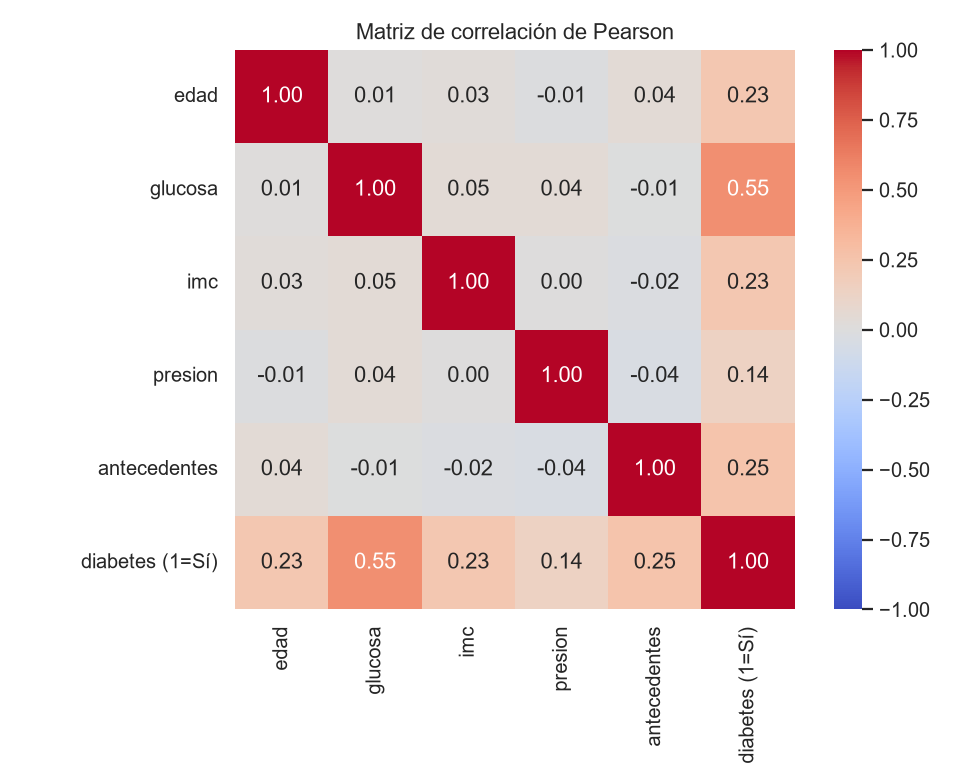
\includegraphics[width=0.48\linewidth]{supervisado/figuras/matriz_correlacion.png}
\caption{Conteo de clases (izq.) y matriz de correlación (der.)}
\end{figure}

\begin{figure}[H]
\centering
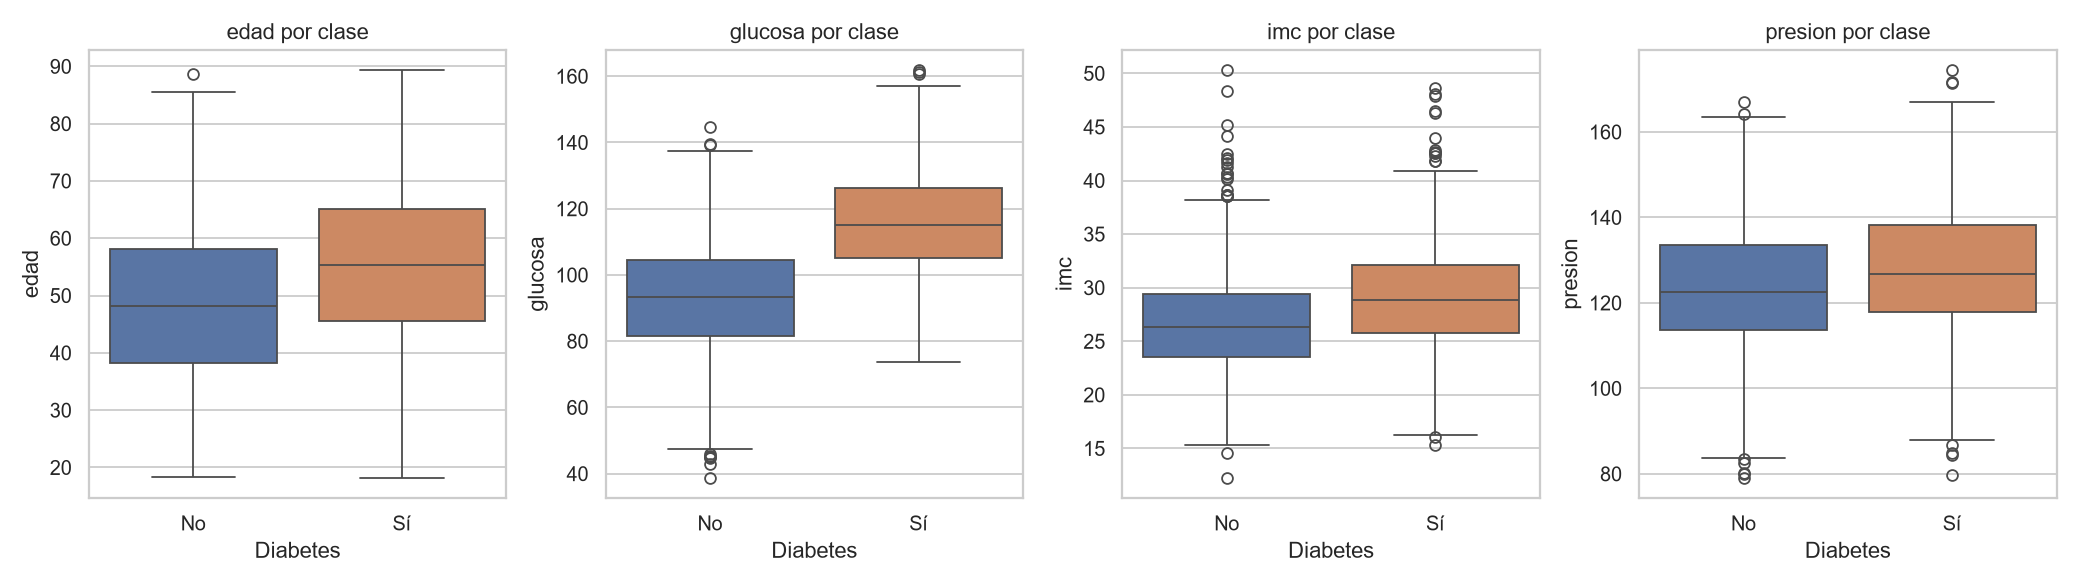
\includegraphics[width=\linewidth]{supervisado/figuras/boxplots_por_clase.png}
\caption{Distribución de las variables según la clase}
\end{figure}

En los diagramas de caja se ve que la glucosa es la variable que más separa a los diabéticos de los que no
lo son, seguida del IMC y la edad. Esto cuadra con la regla, porque la glucosa es la que más pesa en $z$
cuando se tiene en cuenta su escala.

\paragraph{Pruebas de bondad de ajuste.} Para comprobar formalmente las distribuciones usé
Kolmogorov-Smirnov contra la distribución teórica exacta, Shapiro-Wilk para normalidad y chi-cuadrado para
la variable binaria.

\begin{table}[H]
\centering
\caption{Pruebas de bondad de ajuste ($\alpha = 0{,}05$; Bonferroni $\alpha = 0{,}0056$)}
\small
\begin{tabular}{llrrcc}
\toprule
\textbf{Variable} & \textbf{Prueba} & \textbf{Estadístico} & \textbf{p-valor} & \textbf{$\alpha=0{,}05$} & \textbf{Bonferroni} \\
\midrule
Edad          & KS vs. normal truncada       & 0,0176 & 0,557  & No rechaza & No rechaza \\
Glucosa       & KS vs. normal                & 0,0179 & 0,540  & No rechaza & No rechaza \\
IMC           & KS vs. lognormal             & 0,0177 & 0,552  & No rechaza & No rechaza \\
Presión       & KS vs. normal                & 0,0363 & 0,010  & Rechaza    & No rechaza \\
Glucosa       & Shapiro-Wilk                 & 0,9990 & 0,361  & No rechaza & No rechaza \\
Presión       & Shapiro-Wilk                 & 0,9983 & 0,039  & Rechaza    & No rechaza \\
ln(IMC)       & Shapiro-Wilk                 & 0,9987 & 0,124  & No rechaza & No rechaza \\
Edad          & Shapiro-Wilk (sin truncar)   & 0,9943 & $<0{,}001$ & Rechaza & Rechaza \\
Antecedentes  & Chi-cuadrado                 & 0,2881 & 0,591  & No rechaza & No rechaza \\
\bottomrule
\end{tabular}
\end{table}

\subsection{Preparación de los datos}

\begin{itemize}
  \item Separé las cinco variables predictoras en $X$ y la etiqueta en $y$ (Sí $=1$, No $=0$).
  \item Dividí en 80\,\% entrenamiento (1.600 registros) y 20\,\% prueba (400) usando
        \texttt{train\_test\_split} con \texttt{stratify=y} y \texttt{random\_state=42}. Al ser estratificada, las dos partes
        quedaron con el mismo 33,3\,\% de casos positivos.
  \item Para la regresión logística estandaricé las variables con \texttt{StandardScaler}, ajustándolo solo
        con los datos de entrenamiento para no filtrar información del conjunto de prueba.
\end{itemize}

\subsection{Algoritmos y parámetros}

\paragraph{Regresión logística.} Es un modelo lineal que estima la probabilidad de que el paciente tenga
diabetes aplicando la sigmoide a una combinación lineal de las variables. Lo usé dentro de un
\texttt{Pipeline} con \texttt{StandardScaler}, con \texttt{C=1.0} (regularización L2), \emph{solver}
\texttt{lbfgs} y \texttt{max\_iter=1000}.

\paragraph{Random Forest.} Es un conjunto de árboles de decisión, cada uno entrenado con una muestra
\emph{bootstrap} de los datos y un subconjunto aleatorio de variables; la predicción final sale por votación.
Usé \texttt{n\_estimators=300}, \texttt{max\_depth=None}, \texttt{min\_samples\_leaf=2},
\texttt{max\_features='sqrt'} y \texttt{bootstrap=True}. No necesita escalar las variables.

\subsection{Resultados}

\begin{table}[H]
\centering
\caption{Métricas sobre el conjunto de prueba (400 pacientes)}
\begin{tabular}{lccccc}
\toprule
\textbf{Modelo} & \textbf{Accuracy} & \textbf{Precision} & \textbf{Recall} & \textbf{F1-score} & \textbf{Acc. entrenamiento} \\
\midrule
Regresión logística & \textbf{0,855} & 0,774 & \textbf{0,797} & \textbf{0,785} & 0,858 \\
Random Forest       & 0,845 & \textbf{0,775} & 0,752 & 0,763 & 0,978 \\
\midrule
\emph{Regla real sin ruido} & 0,845 & 0,752 & 0,797 & 0,774 & -- \\
\bottomrule
\end{tabular}
\end{table}

\begin{figure}[H]
\centering
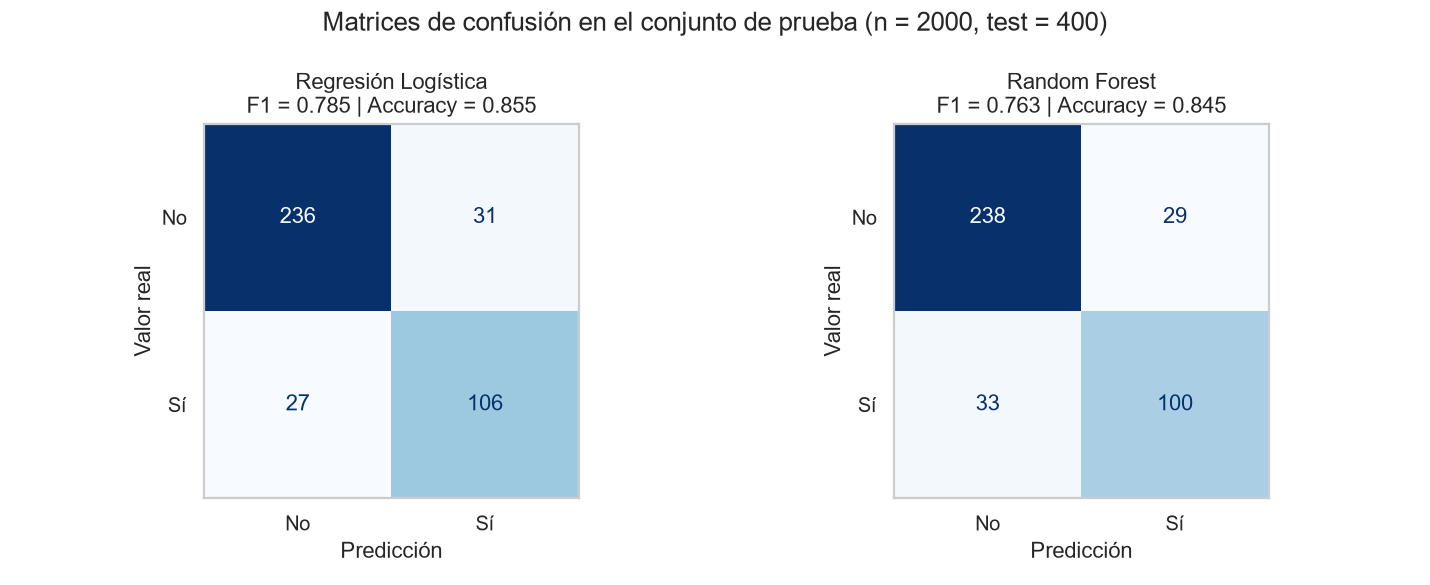
\includegraphics[width=0.9\linewidth]{supervisado/figuras/matrices_confusion.png}
\caption{Matrices de confusión en el conjunto de prueba}
\end{figure}

\begin{table}[H]
\centering
\caption{Matrices de confusión (filas: real; columnas: predicho)}
\begin{tabular}{lcccc}
\toprule
\textbf{Modelo} & \textbf{VN} & \textbf{FP} & \textbf{FN} & \textbf{VP} \\
\midrule
Regresión logística & 236 & 31 & 27 & 106 \\
Random Forest       & 238 & 29 & 33 & 100 \\
\bottomrule
\end{tabular}
\end{table}

\begin{figure}[H]
\centering
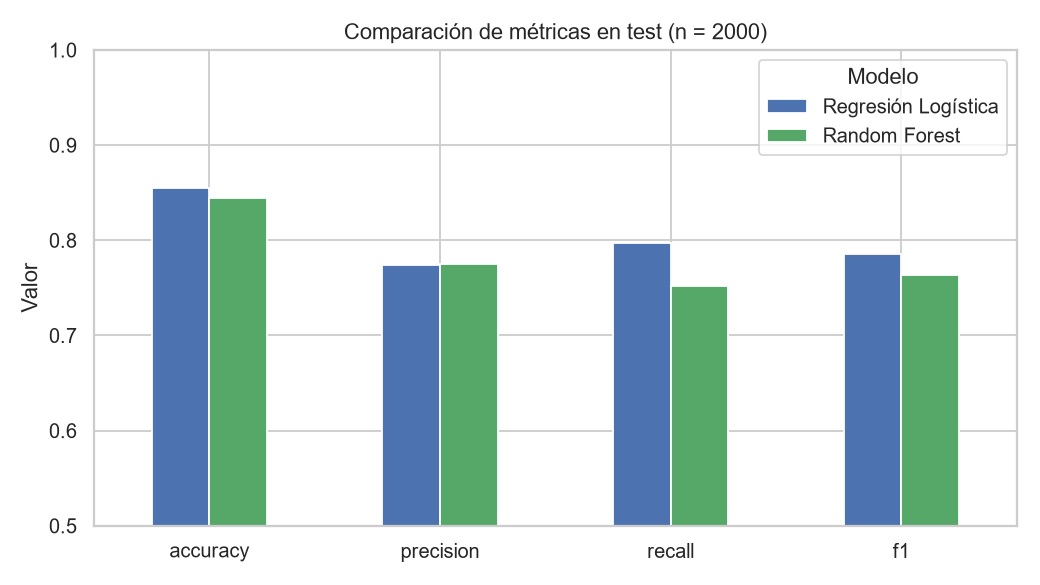
\includegraphics[width=0.48\linewidth]{supervisado/figuras/comparacion_metricas.png}
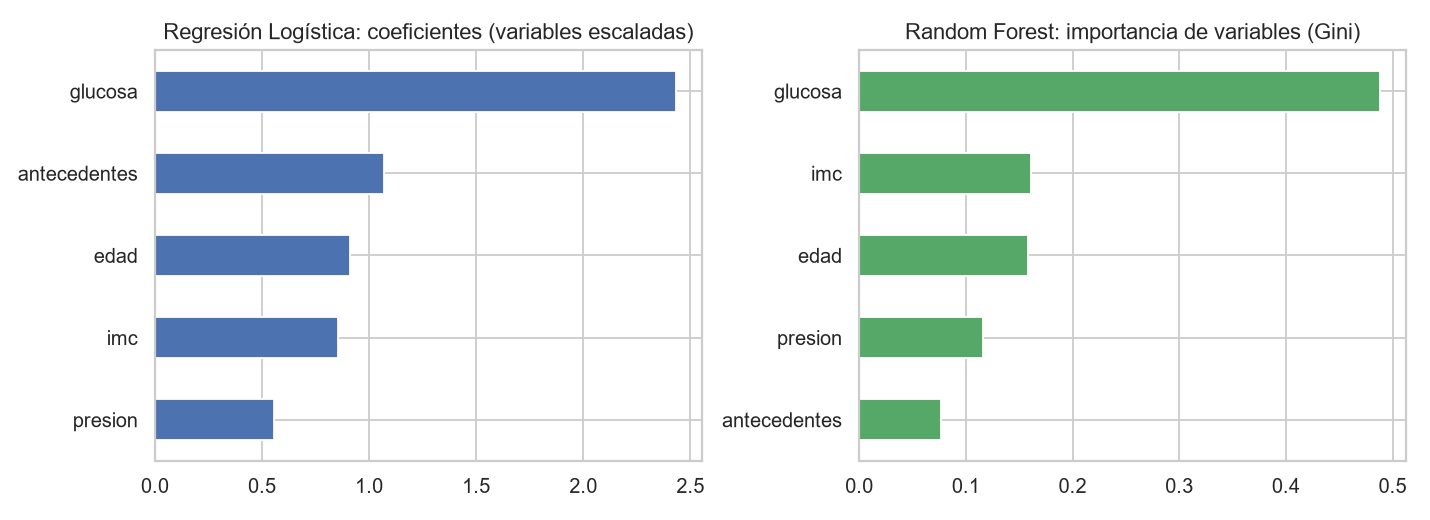
\includegraphics[width=0.48\linewidth]{supervisado/figuras/importancia_variables.png}
\caption{Comparación de métricas (izq.) e importancia de variables en Random Forest (der.)}
\end{figure}

La importancia de variables del Random Forest confirma lo que se veía en el análisis exploratorio: la
glucosa pesa casi la mitad (0,49), y luego vienen IMC (0,16), edad (0,16), presión (0,12) y antecedentes (0,08).

\subsection{Efecto del tamaño del conjunto de datos}

Repetí todo el proceso con 500, 2.000 y 10.000 registros, cinco veces por tamaño con semillas distintas,
y promedié las métricas.

\begin{table}[H]
\centering
\caption{Métricas promedio según el número de registros (media de 5 repeticiones)}
\small
\begin{tabular}{rlccccc}
\toprule
\textbf{$n$} & \textbf{Modelo} & \textbf{Accuracy} & \textbf{Precision} & \textbf{Recall} & \textbf{F1 ($\pm$ desv.)} & \textbf{Acc. entren.} \\
\midrule
500    & Regresión logística & 0,834 & 0,764 & 0,715 & 0,737 $\pm$ 0,047 & 0,861 \\
500    & Random Forest       & 0,802 & 0,712 & 0,667 & 0,685 $\pm$ 0,058 & 0,983 \\
2.000  & Regresión logística & 0,853 & 0,801 & 0,746 & 0,771 $\pm$ 0,023 & 0,849 \\
2.000  & Random Forest       & 0,837 & 0,774 & 0,721 & 0,745 $\pm$ 0,020 & 0,976 \\
10.000 & Regresión logística & 0,845 & 0,792 & 0,729 & 0,759 $\pm$ 0,009 & 0,851 \\
10.000 & Random Forest       & 0,834 & 0,770 & 0,718 & 0,743 $\pm$ 0,011 & 0,978 \\
\bottomrule
\end{tabular}
\end{table}

\begin{figure}[H]
\centering
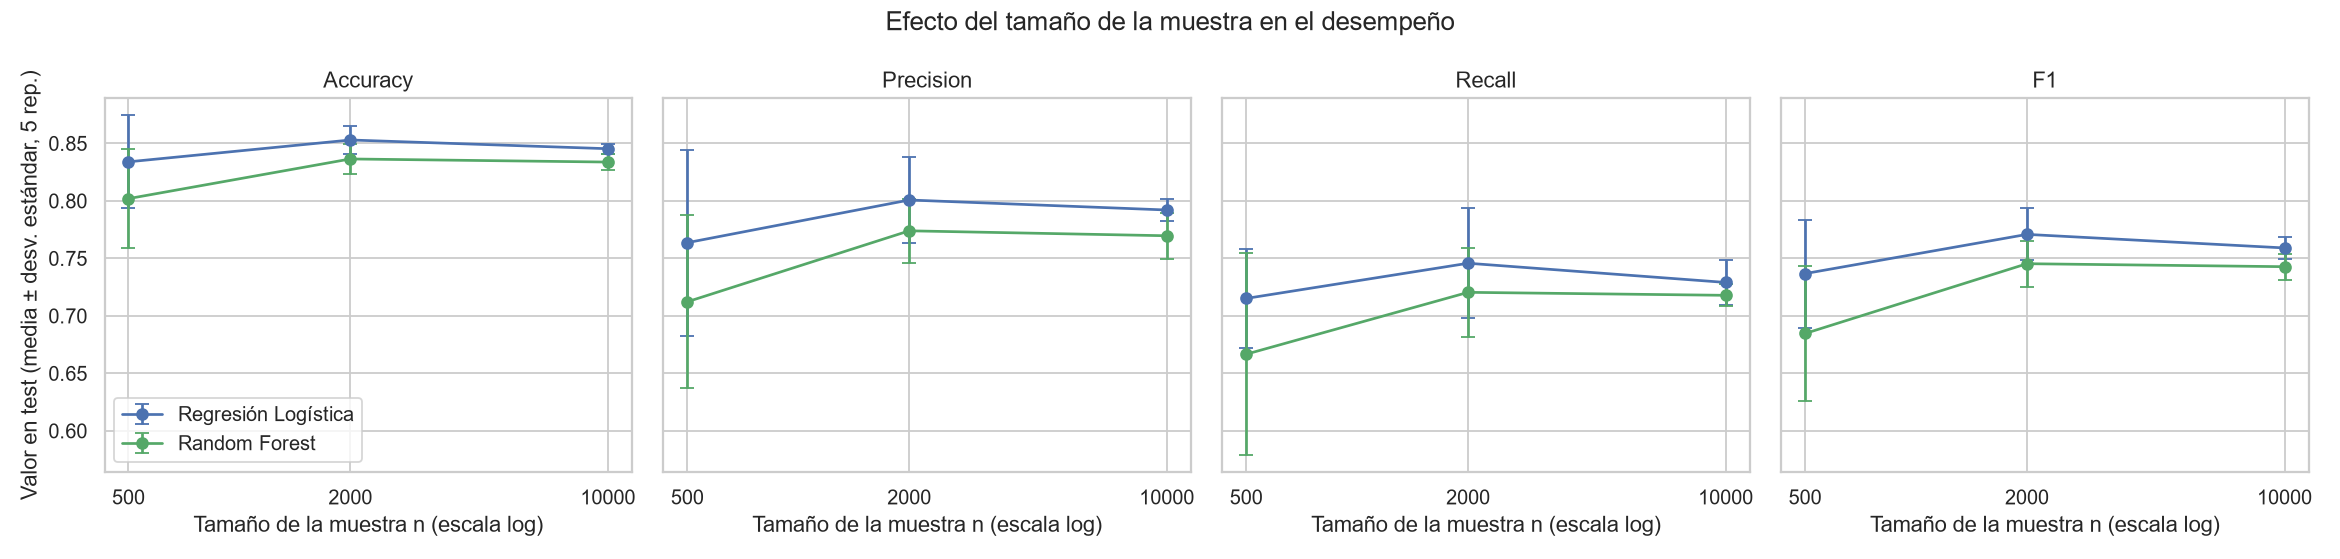
\includegraphics[width=0.85\linewidth]{supervisado/figuras/experimento_tamano.png}
\caption{Métricas en función del número de registros}
\end{figure}

\subsection{Respuestas a las preguntas}

\paragraph{1. ¿Las variables generadas siguen las distribuciones estadísticas esperadas?}
Sí. Para edad, glucosa, IMC y antecedentes ninguna prueba rechaza la hipótesis de que siguen la distribución
teórica, y los histogramas coinciden muy bien con las curvas. La presión arterial dio $p = 0{,}010$ en KS y
$0{,}039$ en Shapiro, lo que a primera vista parecería un rechazo. Pero como hice nueve pruebas a la vez, lo
correcto es aplicar la corrección de Bonferroni ($\alpha = 0{,}0056$), y con eso ya no se rechaza. Además, la
presión se generó exactamente con una normal, así que ese resultado es un error tipo I, algo que pasa
aproximadamente una de cada veinte veces por puro azar. La edad no pasa la prueba de normalidad
\emph{sin truncar}, pero eso era lo esperado porque la corté entre 18 y 90 años; contra la normal truncada sí
se ajusta.

\paragraph{2. ¿Qué proporción de pacientes pertenece a cada clase?}
1.333 pacientes sin diabetes (66,65\,\%) y 667 con diabetes (33,35\,\%). Es un desbalance moderado de más o
menos 2 a 1, y por eso fue importante usar la división estratificada.

\paragraph{3. ¿Cuál de los algoritmos obtiene el mejor F1-score?}
La regresión logística, con F1 $= 0{,}785$ frente a $0{,}763$ del Random Forest. También gana en accuracy y
recall; en precisión quedan prácticamente empatados. Su F1 queda incluso a la par de la regla real sin ruido
($0{,}774$), o sea que llegó prácticamente al techo que permiten los datos.

\paragraph{4. ¿Qué sucede cuando se cambia el número de registros de 500 a 2.000 o 10.000?}
De 500 a 2.000 los dos modelos mejoran, sobre todo el Random Forest (su F1 sube de 0,685 a 0,745), porque
es un modelo más flexible que necesita más ejemplos. De 2.000 a 10.000 las métricas prácticamente no cambian:
el límite ya no lo pone la cantidad de datos, sino el ruido de la etiqueta. Lo que sí mejora bastante es la
estabilidad: la desviación del F1 baja de cerca de 0,05 a cerca de 0,01, es decir, con más datos los resultados
dependen mucho menos de qué pacientes caigan en la prueba. También se ve que el Random Forest sobreajusta en
todos los tamaños (alrededor de 0,98 en entrenamiento contra 0,83 en prueba).

\paragraph{5. ¿Qué ventajas y desventajas presenta cada algoritmo?}
En la Tabla~\ref{tab:ventajas} resumo lo que observé de cada uno en esta actividad.

\begin{table}[H]
\centering
\caption{Ventajas y desventajas de cada algoritmo}
\label{tab:ventajas}
\small
\begin{tabularx}{\linewidth}{lXX}
\toprule
& \textbf{Ventajas} & \textbf{Desventajas} \\
\midrule
\textbf{Regresión logística} &
Es simple, rápida e interpretable: los coeficientes dicen cuánto pesa cada variable. Entrega probabilidades
bien calibradas, casi no sobreajusta y funciona bien con pocos datos. &
Asume que la frontera de decisión es lineal, así que no capta interacciones ni relaciones no lineales a menos
que uno las construya a mano. Requiere escalar las variables. \\
\addlinespace
\textbf{Random Forest} &
Capta relaciones no lineales e interacciones sin tener que especificarlas, no necesita escalado, es robusto
a datos atípicos y da la importancia de cada variable. &
Es más pesado de entrenar y mucho menos interpretable. Tiende a memorizar el ruido (sobreajuste) y necesita
más datos para rendir bien. \\
\bottomrule
\end{tabularx}
\end{table}

% ================================================================== PARTE 2
\newpage
\section{Parte 2: ML no supervisado -- segmentación de clientes}

\subsection{Descripción del problema}

Aquí el objetivo es distinto: no hay una etiqueta que predecir. Generé 3.200 clientes de un supermercado con
su edad, ingresos anuales, frecuencia de compra mensual, valor promedio del tiquete y gasto mensual, y la
idea es que los algoritmos encuentren por sí solos grupos de clientes parecidos. Usé K-means, K-medoids y
clustering jerárquico.

\subsection{Distribuciones seleccionadas}

Para que existieran grupos reales que encontrar, generé los datos como una mezcla de cuatro segmentos. La
etiqueta del segmento \textbf{no} se le pasa a ningún algoritmo; solo la guardé para comprobar al final qué
tan bien se recuperaron los grupos (con el índice ARI).

\begin{table}[H]
\centering
\caption{Parámetros de los segmentos latentes}
\footnotesize
\setlength{\tabcolsep}{3.5pt}
\begin{tabular}{lrllll}
\toprule
\textbf{Segmento} & \textbf{$n$} & \textbf{Edad} & \textbf{Ingresos (lognormal)} & \textbf{Visitas (Poisson)} & \textbf{Tiquete (gamma)} \\
\midrule
Jóvenes/estudiantes   & 800   & Uniforme(18, 28) & med. 14.000, $\sigma=0{,}35$ & $\lambda=5$  & $(4;\ 5)$ \\
Familias              & 1.000 & Normal(42, 6)    & med. 38.000, $\sigma=0{,}30$ & $\lambda=14$ & $(6;\ 9)$ \\
Profesionales premium & 600   & Normal(33, 4)    & med. 90.000, $\sigma=0{,}25$ & $\lambda=3$  & $(6;\ 18)$ \\
Adultos mayores       & 800   & Normal(68, 5)    & med. 22.000, $\sigma=0{,}30$ & $\lambda=16$ & $(5;\ 3{,}5)$ \\
\bottomrule
\end{tabular}
\end{table}

Los ingresos son lognormales porque el dinero siempre es positivo y tiene cola larga a la derecha; la
frecuencia es Poisson porque es un conteo de visitas; y el tiquete es gamma por ser positivo y asimétrico.
El tiquete se multiplica por $(\text{ingresos}/\text{mediana})^{0,3}$ para que la gente con más plata gaste
un poco más por visita, y el gasto mensual es $\text{frecuencia} \times \text{tiquete} \times \mathcal{N}(1;\,0{,}05)$.

\subsection{Código utilizado para generar los datos}

\lstinputlisting[firstline=46,lastline=95]{../no_supervisado/no_supervisado.py}

\subsection{Análisis exploratorio}

\begin{table}[H]
\centering
\caption{Estadísticas descriptivas ($n = 3.200$)}
\small
\begin{tabular}{lrrrrrrr}
\toprule
\textbf{Variable} & \textbf{Media} & \textbf{Desv.} & \textbf{Mín.} & \textbf{Mediana} & \textbf{Máx.} & \textbf{Asim.} & \textbf{Curt.} \\
\midrule
Edad (años)             & 41,9    & 17,2    & 18     & 38     & 83      & 0,55 & $-0{,}96$ \\
Ingresos (USD/año)      & 39.579  & 31.204  & 3.904  & 28.158 & 172.657 & 1,51 & 1,66 \\
Frecuencia (visitas/mes)& 10,1    & 6,3     & 1      & 10     & 31      & 0,27 & $-0{,}95$ \\
Tiquete (USD)           & 47,5    & 42,8    & 2,1    & 31,6   & 374,2   & 1,76 & 3,79 \\
Gasto (USD/mes)         & 393,2   & 361,0   & 4,5    & 284,9  & 3.112,3 & 1,78 & 4,55 \\
\bottomrule
\end{tabular}
\end{table}

\begin{figure}[H]
\centering
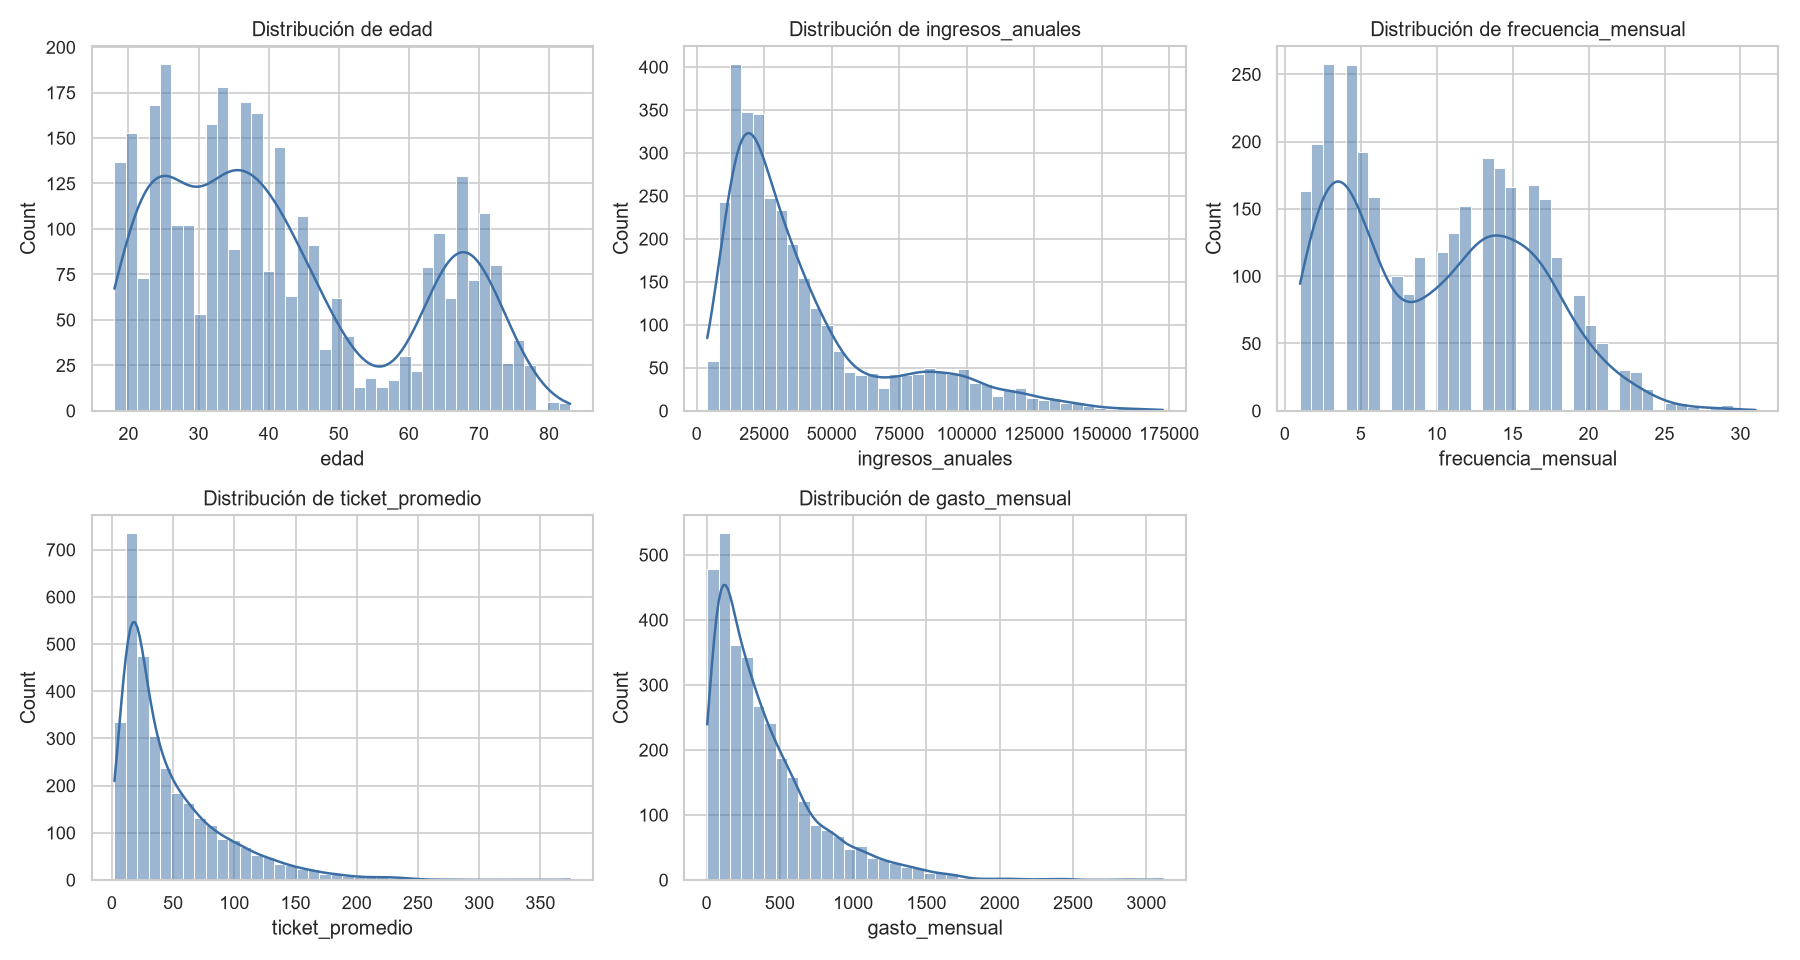
\includegraphics[width=\linewidth]{no_supervisado/figuras/01_histogramas.png}
\caption{Histogramas de las variables de clientes}
\end{figure}

\begin{figure}[H]
\centering
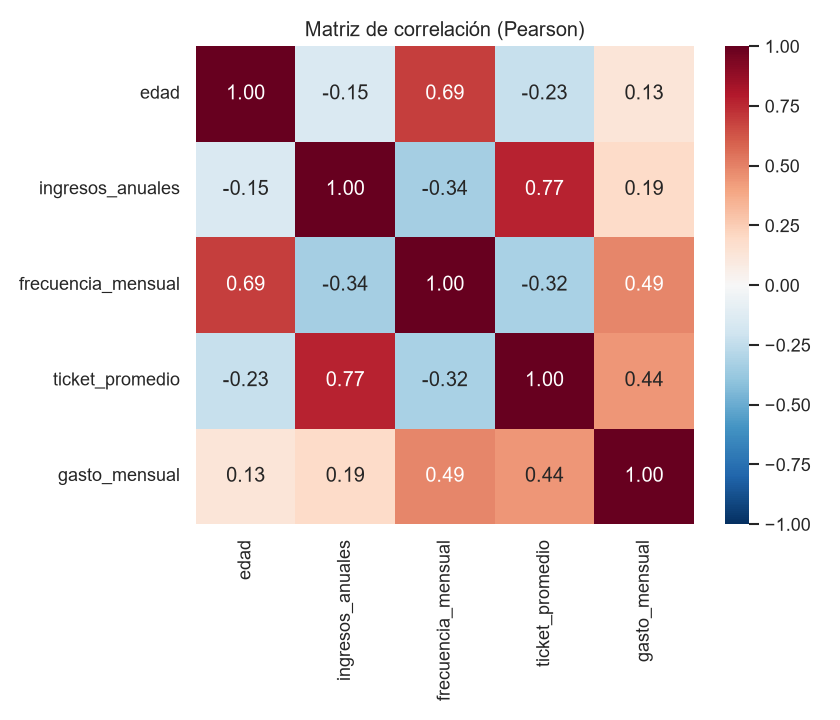
\includegraphics[width=0.48\linewidth]{no_supervisado/figuras/03_correlaciones.png}
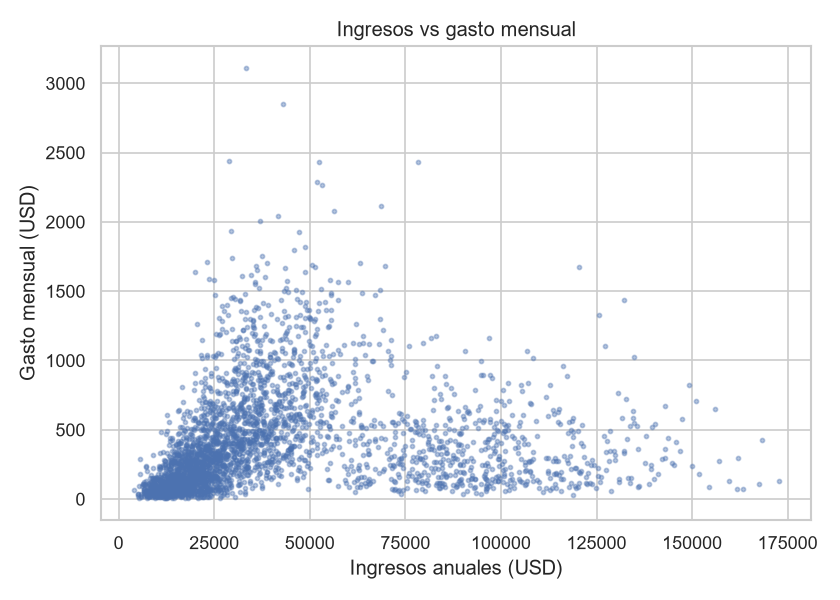
\includegraphics[width=0.48\linewidth]{no_supervisado/figuras/05_scatter_ingresos_gasto.png}
\caption{Matriz de correlación (izq.) y relación ingresos--gasto (der.)}
\end{figure}

Ingresos, tiquete y gasto tienen una asimetría fuerte (entre 1,5 y 1,8), así que antes de agrupar les apliqué
$\log(1+x)$ y luego estandaricé todo con \texttt{StandardScaler}. Si no se hace esto, los algoritmos basados en
distancias quedan dominados por las variables de dinero, que tienen escalas mucho más grandes. Las
correlaciones más fuertes fueron ingresos--tiquete (0,77) y edad--frecuencia (0,69).

\subsection{Algoritmos y parámetros}

\begin{itemize}
  \item \textbf{K-means:} \texttt{KMeans(n\_clusters=k, n\_init=10, random\_state=42)}. Asigna cada cliente al
        centroide más cercano y minimiza la inercia (suma de distancias al cuadrado).
  \item \textbf{K-medoids:} lo implementé directamente en NumPy porque la librería \texttt{scikit-learn-extra}
        no se pudo instalar en la versión de Python que estaba usando. Usa una inicialización tipo
        \emph{k-medoids++}, alterna entre asignar clientes y actualizar medoides, y hace 5 reinicios. La
        diferencia con K-means es que los centros son clientes reales, lo que lo hace más robusto a atípicos.
  \item \textbf{Jerárquico aglomerativo:} \texttt{AgglomerativeClustering(n\_clusters=k, linkage='ward')}.
        Empieza con cada cliente como un grupo y los va uniendo minimizando el aumento de varianza.
        El dendrograma lo dibujé con una muestra de 300 clientes para que se pudiera leer.
\end{itemize}

\subsection{Selección del número de grupos}

\begin{figure}[H]
\centering
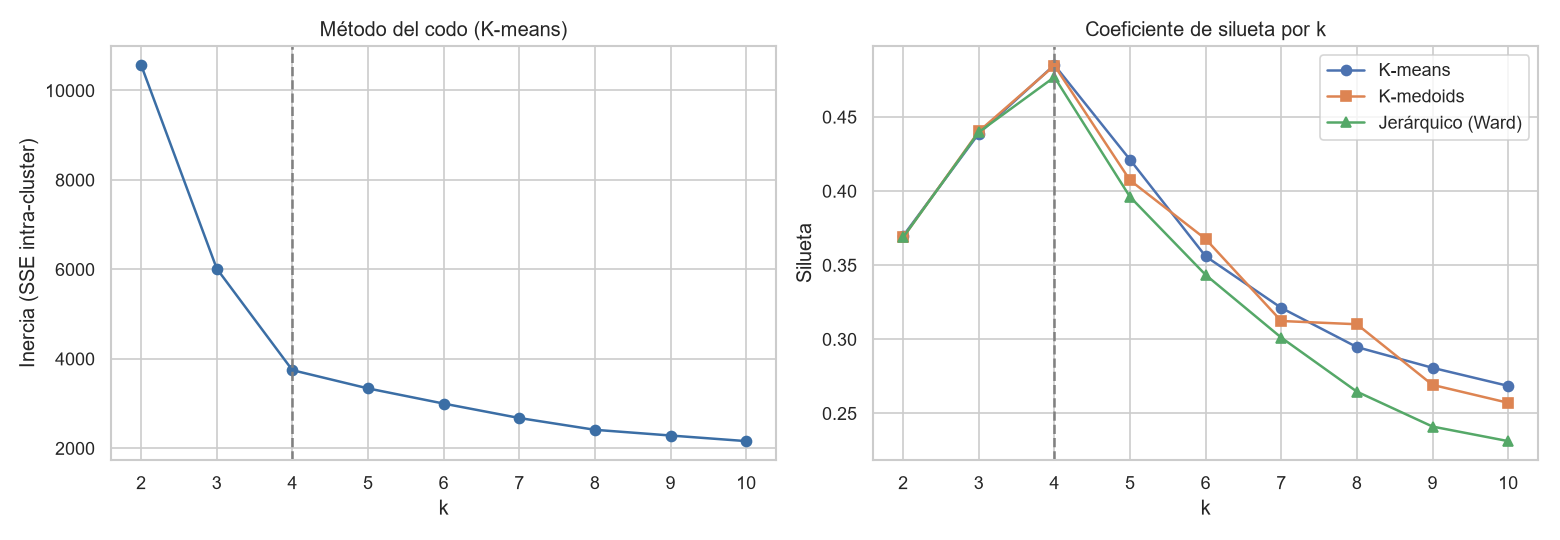
\includegraphics[width=0.95\linewidth]{no_supervisado/figuras/06_codo_silueta.png}
\caption{Método del codo (inercia) y coeficiente de silueta para $k = 2, \dots, 10$}
\end{figure}

La inercia baja fuerte hasta $k=4$ (10.569 $\rightarrow$ 6.016 $\rightarrow$ 3.745) y de ahí en adelante baja
poquito (3.337 en $k=5$), así que el codo está en 4. La silueta también es máxima en $k=4$ para los tres
algoritmos (0,485 en K-means). Como los dos criterios coinciden, escogí $k = 4$, que además es el número
real de segmentos con los que generé los datos.

\begin{figure}[H]
\centering
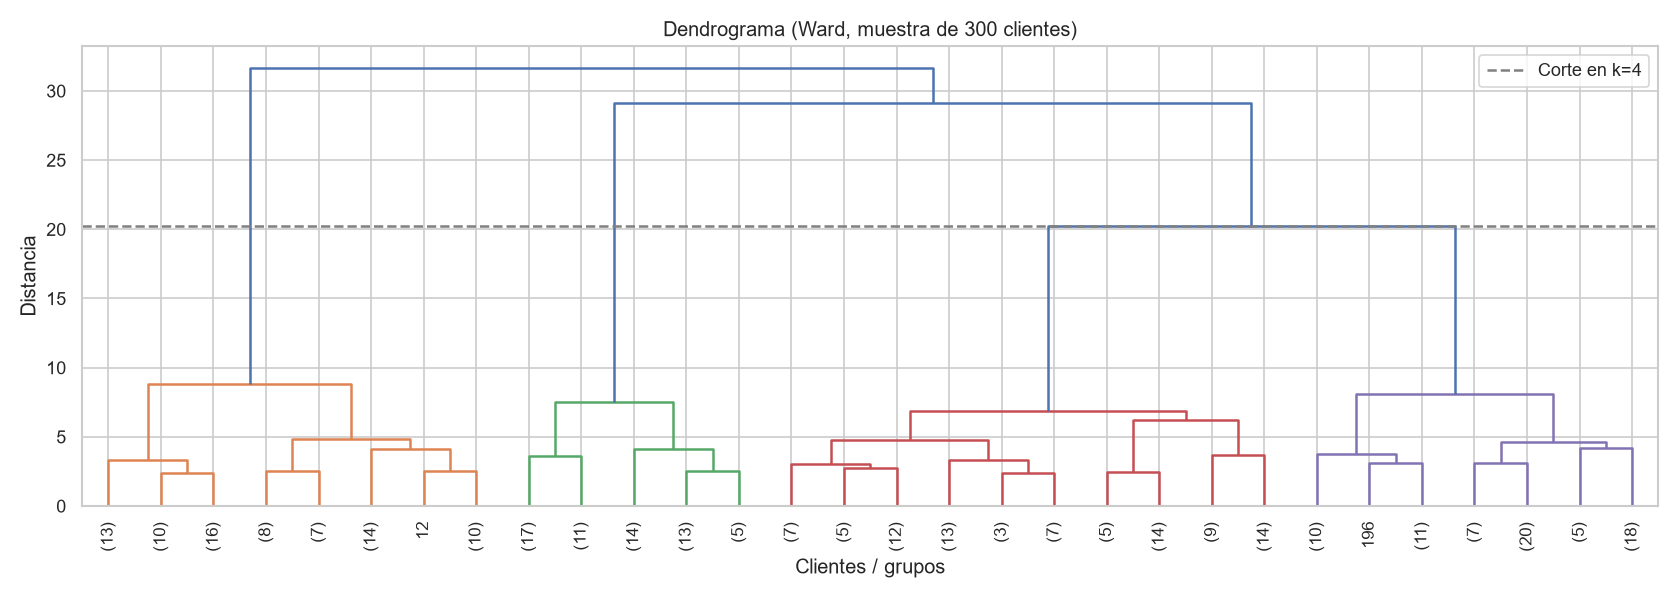
\includegraphics[width=0.85\linewidth]{no_supervisado/figuras/09_dendrograma.png}
\caption{Dendrograma del clustering jerárquico (Ward, muestra de 300 clientes)}
\end{figure}

\subsection{Comparación de los algoritmos}

\begin{table}[H]
\centering
\caption{Métricas de calidad con $k = 4$}
\begin{tabular}{lcccc}
\toprule
\textbf{Algoritmo} & \textbf{Silueta} $\uparrow$ & \textbf{Davies-Bouldin} $\downarrow$ & \textbf{Calinski-Harabasz} $\uparrow$ & \textbf{ARI vs. real} $\uparrow$ \\
\midrule
K-means           & \textbf{0,485} & 0,766 & \textbf{3.486} & 0,946 \\
K-medoids         & 0,485 & \textbf{0,762} & 3.474 & 0,940 \\
Jerárquico (Ward) & 0,477 & 0,782 & 3.359 & \textbf{0,964} \\
\bottomrule
\end{tabular}
\end{table}

\begin{figure}[H]
\centering
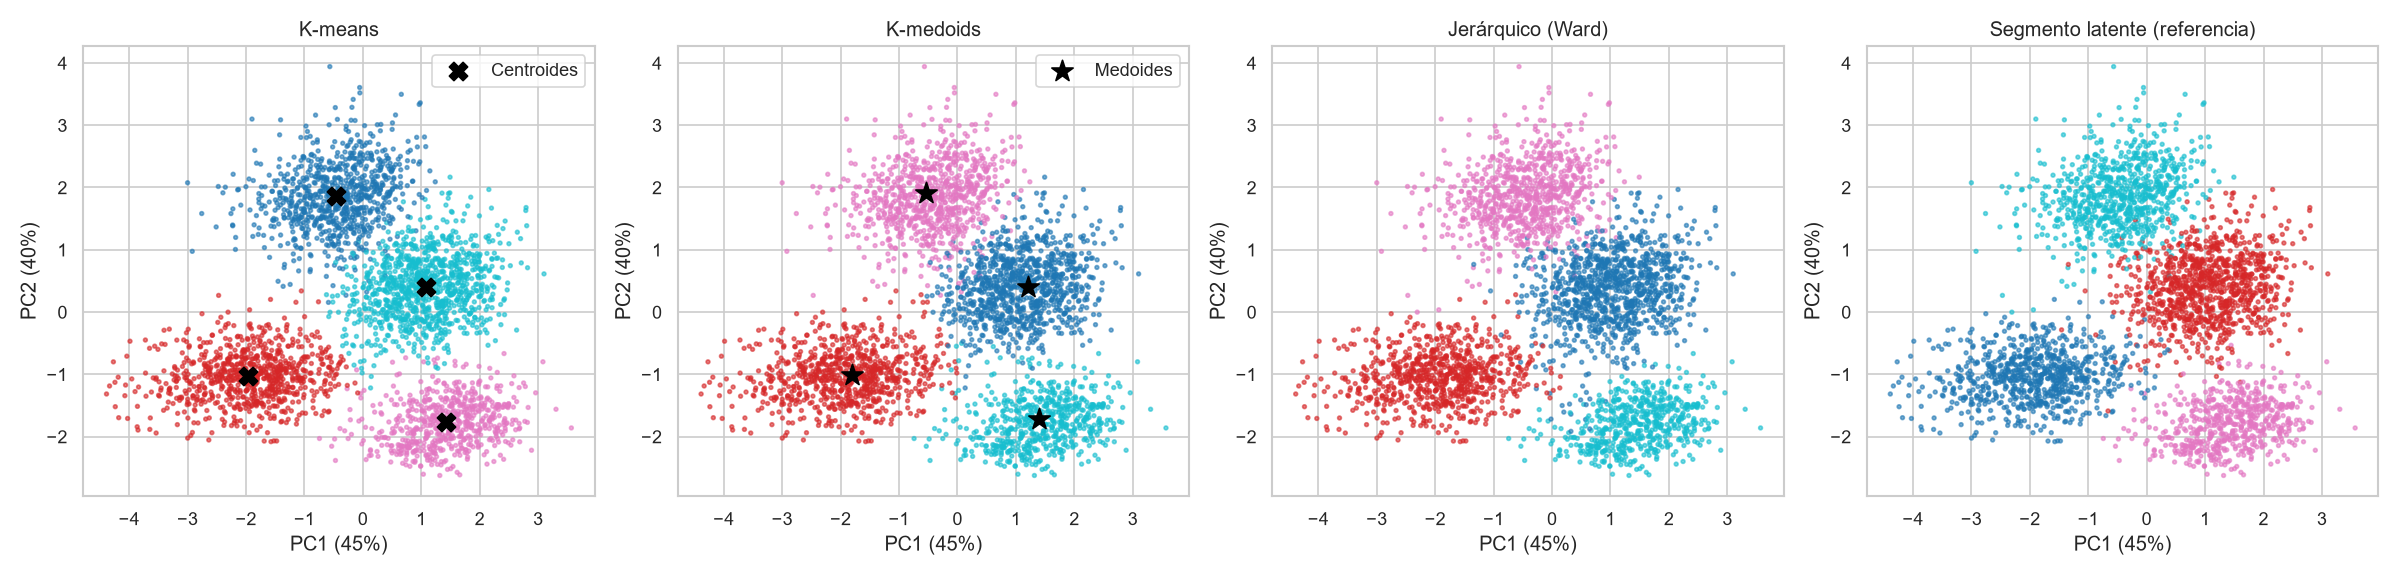
\includegraphics[width=\linewidth]{no_supervisado/figuras/08_pca_clusters.png}
\caption{Clusters de cada algoritmo proyectados en 2D con PCA (85\,\% de la varianza)}
\end{figure}

\subsection{Interpretación de los clusters}

\begin{table}[H]
\centering
\caption{Promedios por cluster (K-means)}
\small
\begin{tabular}{clrrrrrr}
\toprule
\textbf{C.} & \textbf{Perfil} & \textbf{Edad} & \textbf{Ingresos} & \textbf{Visitas} & \textbf{Tiquete} & \textbf{Gasto} & \textbf{\%} \\
\midrule
0 & Adultos mayores       & 67,5 & 23.037 & 16,0 & 17,6  & 282 & 25,4 \\
1 & Jóvenes/estudiantes   & 23,2 & 14.738 & 4,8  & 19,5  & 93  & 24,8 \\
2 & Profesionales premium & 33,2 & 94.361 & 3,1  & 112,1 & 343 & 19,1 \\
3 & Familias              & 41,4 & 39.281 & 13,8 & 54,8  & 758 & 30,8 \\
\bottomrule
\end{tabular}
\end{table}

\begin{figure}[H]
\centering
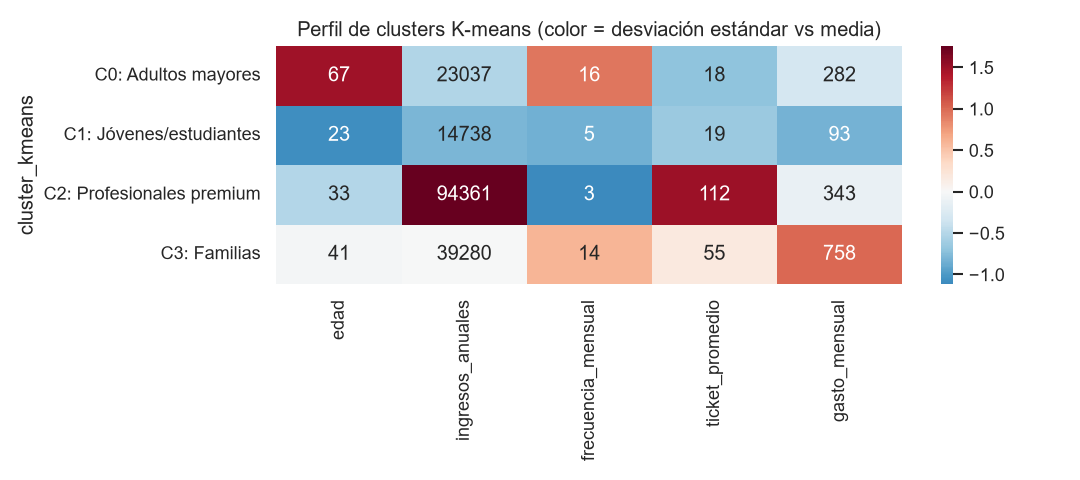
\includegraphics[width=0.8\linewidth]{no_supervisado/figuras/10_perfiles_heatmap.png}
\caption{Perfil promedio estandarizado de cada cluster}
\end{figure}

\begin{itemize}
  \item \textbf{Adultos mayores (25\,\%):} van al supermercado casi todos los días (16 veces al mes), pero
        compran poquito en cada visita. Ingresos medios-bajos.
  \item \textbf{Jóvenes/estudiantes (25\,\%):} los de menores ingresos y menor gasto; van pocas veces y con
        tiquetes pequeños.
  \item \textbf{Profesionales premium (19\,\%):} los de mayores ingresos. Van muy poco (3 veces al mes), pero
        cada compra es grande (más de 110 USD).
  \item \textbf{Familias (31\,\%):} el grupo más valioso para el supermercado, porque combinan buena frecuencia
        con un tiquete medio y terminan siendo los que más gastan al mes (758 USD).
\end{itemize}

\subsection{Respuestas a las preguntas}

\paragraph{1. ¿Qué resultados obtuvo?}
Sin usar ninguna etiqueta, los tres algoritmos encontraron prácticamente los mismos cuatro grupos, con una
calidad de agrupamiento entre moderada y buena (silueta alrededor de 0,48 y Davies-Bouldin alrededor de 0,76).
K-means y K-medoids quedaron casi empatados y coinciden entre sí en un 97,6\,\% (ARI), mientras que el
jerárquico con Ward fue el que mejor recuperó los segmentos reales (ARI de 0,964). Las variables que más
diferencian a los grupos son la edad, la frecuencia de visita y el valor del tiquete.

\paragraph{2. ¿Para qué serviría este análisis?}
Para segmentar clientes y tomar decisiones de mercadeo y operación:
\begin{itemize}
  \item Hacer promociones dirigidas: descuentos por volumen para las familias, productos gourmet o domicilios
        para los profesionales premium, beneficios de fidelidad en horas de poca afluencia para los adultos
        mayores y marca propia o precios bajos para los jóvenes.
  \item Ajustar el surtido de productos y el personal según los horarios de cada grupo.
  \item Diseñar programas de lealtad diferenciados.
  \item Identificar segmentos con riesgo de dejar de comprar o con potencial de gastar más.
  \item Asignar automáticamente a un cliente nuevo al segmento que le corresponde, sin etiquetarlo a mano.
\end{itemize}

% ================================================================== CONCLUSIONES
\newpage
\section{Conclusiones}

\begin{itemize}
  \item En la parte supervisada el mejor modelo fue la \textbf{regresión logística} (F1 $=0{,}785$ contra
        $0{,}763$). La razón principal es que la etiqueta se construyó con una regla lineal pasada por una
        sigmoide, que es exactamente la forma del modelo logístico. El Random Forest, al ser más flexible,
        terminó aprendiéndose parte del ruido: casi 0,98 de accuracy en entrenamiento pero 0,85 en prueba.
  \item El rendimiento de cualquier modelo queda limitado por el ruido que se le metió a la etiqueta. Ninguno
        puede superar por mucho a la regla verdadera sin ruido, y por eso pasar de 2.000 a 10.000 registros
        no sube las métricas, solo las hace más estables.
  \item Si la regla de diabetes hubiera tenido interacciones o relaciones no lineales (por ejemplo, que la
        glucosa solo importe a partir de cierta edad), muy probablemente el Random Forest le hubiera ganado a
        la regresión logística. La elección del modelo depende de la forma real del problema.
  \item En la parte no supervisada, el método del codo y la silueta coincidieron en $k=4$, que es justo el
        número de segmentos con el que se generaron los datos. Los tres algoritmos llegaron a grupos casi
        idénticos: K-means es el más rápido, K-medoids da centros que son clientes reales y es más robusto a
        atípicos, y el jerárquico con Ward recuperó mejor la estructura original y además permite ver la
        jerarquía en el dendrograma.
  \item Un aprendizaje práctico fue la importancia del preprocesamiento: sin la transformación logarítmica y
        la estandarización de las variables de dinero, los grupos no salían tan bien definidos.
\end{itemize}

\end{document}
